% @Author: AnthonyKenny98
% @Date:   2020-02-23 12:45:54
% @Last Modified by:   AnthonyKenny98
% @Last Modified time: 2020-02-23 14:25:32

\subsection{Background}
    \todo[inline]{TODO: Summarize the following points: \\ 
        1) Need for faster execution of motion planning in drones \\
        2) Strategy of specialized hardware \\
        3) RISC-V ISA and its potentials including extendibility \\
    }

    \subsubsection*{Robotics}
        For well over 2000 years, the concept of robotics, albeit not always with such a term, has fascinated humans. As early as the first century A.D., the Greek mathematician and engineer, Heron of Alexandria, described more than 100 different machines and automata in \textit{Pneumatica} and \textit{Automata}\cite{Alexandrinus}. In 1898, Nikola Tesla demonstrated the first radio-controlled vessel. Since then, the world has seen widespread application of robotics in manufacturing, mining, transport, exploration, and weaponry. For the last few decades, robots have operated in controlled, largely unchanging environments (e.g.\ an assembly line) where their environment and movements are largely known \textit{a priori}.
        \newline
        However, in recent years a new generation of autonomous robots has been developed for a wide range of real-world, complex applications. The increasing trend the use of autonomous robots is shown in Figure \ref{fig:useOfAutonomousRobots}. These new robots, unlike those traditional ones described above, are required to adapt to the changing environment in which they operate. As such, they must perform motion planning in real time.

        % @Author: AnthonyKenny98
% @Date:   2020-02-23 12:12:56
% @Last Modified by:   AnthonyKenny98
% @Last Modified time: 2020-02-23 13:56:51

\begin{figure}%[H]
\begin{center}
\missingfigure[figwidth=\linewidth]{Some sort of line/bar graph showing the increasing use of Autonomous robots over time. Need to find}
% 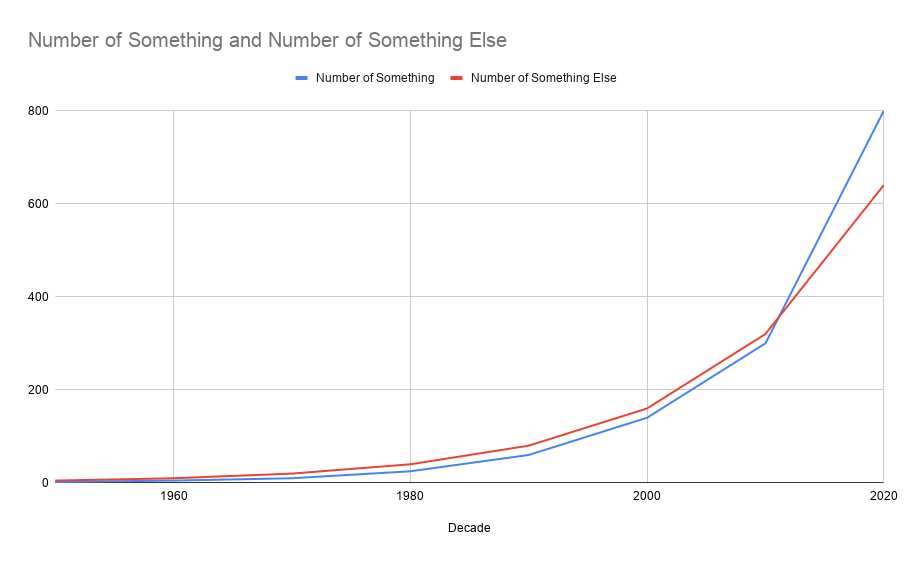
\includegraphics[width=0.8\linewidth]{img/sampleLineGraph.png}
\caption{The use of Autonomous Robots over time}
\label{fig:useOfAutonomousRobots}
\end{center}
\end{figure}

    \subsubsection*{Motion Planning}
        \todo[inline]{TODO: More of an introduction to motion planning.}
        
        Motion Planning refers to the problem of determining how a robot moves through a space to acheive a goal. Chapter \ref{chap:MotionPlanningInSoftware} provides a detailed explanation of motion planning and of \ac{RRT}, a commonly used motion planning algorithm.
        \newline
        On the algorithmic level, motion planning has been extensively studied and many solutions exist. However, current algorithms running on regular \ac{CPU}s are too slow to execute in real time for robots operating in complex environments. Simply solving this problem with more raw computing power, using energy hungry \ac{GPU}s may have merit in tethered robots. On the other hand, untethered applications, such as autonomous drones, where limiting power consumption is a primary concern, this strategy is infeasible.
        
    \subsection*{Hardware Acceleration}
        Specialized hardware designed to perform specific functions can yield significantly higher performance than software running on general purpose processors, and lower power consumption than \ac{GPU}s.
        \todo[inline]{More detail here. Reference prior work}

    \subsubsection{RISC-V}
        \todo[inline]{TODO: Introduction to RISC-V and its merits in this problem}


\subsection{Problem Definition}

    \subsubsection*{Problem Statement}
    \todo[inline]{Revise problem statement}
    Current processors cannot compute motion planning algorithms quickly enough for robots to operate in high complexity environments. Autonomous drones are a specific case of robots requiring real-time motion planning in complex environments. The state-of-the-art strategy of using a Graphics Processing Unit (GPU) to accelerate the execution of these algorithms requires too much power to be cost-effective or feasible for drones to sustain flight for useful periods of time.

    \subsubsection*{End User}
    \todo[inline]{TODO: End User}